
\chapter{Linear independence}

\index{linear independence}

One of the deepest and most central concepts in linear algebra -- in fact, if I
were to make a top ten ranking, this one might just make \#1 -- is that of
\textbf{linear independence}. It's not about mechanical computations, but
conceptual truths. Learn this chapter well. 

\section{The Domino Game}
\index{the Domino Game}

I've thought long and hard about the best way to teach the material in this
chapter, and I've come up with a game. I call it ``the Domino Game.'' Here are
the rules:

\begin{framed}
\begin{compactenum}
\item You are given one or more yellow\footnotemark ``starter dominos.''
\item The object of the game is to build the white ``goal domino'' from these
starter dominos.
\item You can ``use'' any number of each starter domino (even a fraction, even
negative), and add them together (left sides add together, and right sides add
together).
\item You \textit{cannot} use only one side of a domino.
\item You \textit{cannot} turn a domino around so the left side and right
sides flip.
\end{compactenum}
\end{framed}

\footnotetext{Gray, actually, since I made this a black and white book to keep costs down.}

Example. Suppose your starter dominos are:

\begin{center}
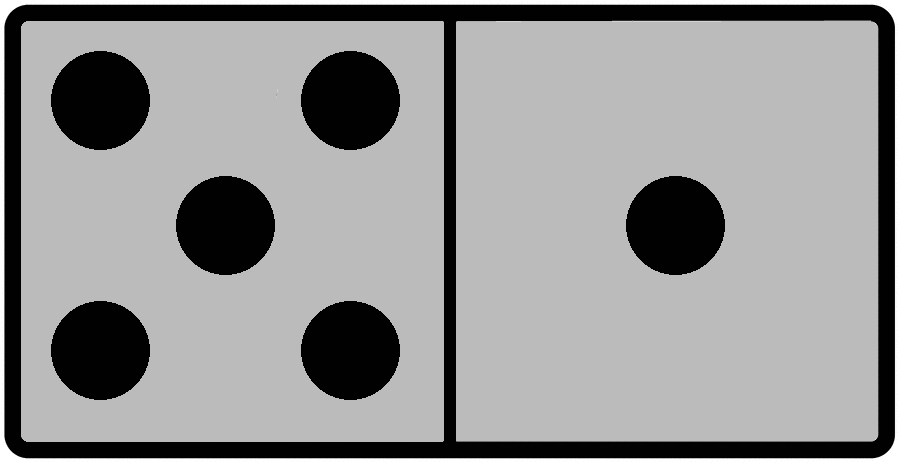
\includegraphics[width=0.3\textwidth]{gray5_1.png}
\hspace{.3in}
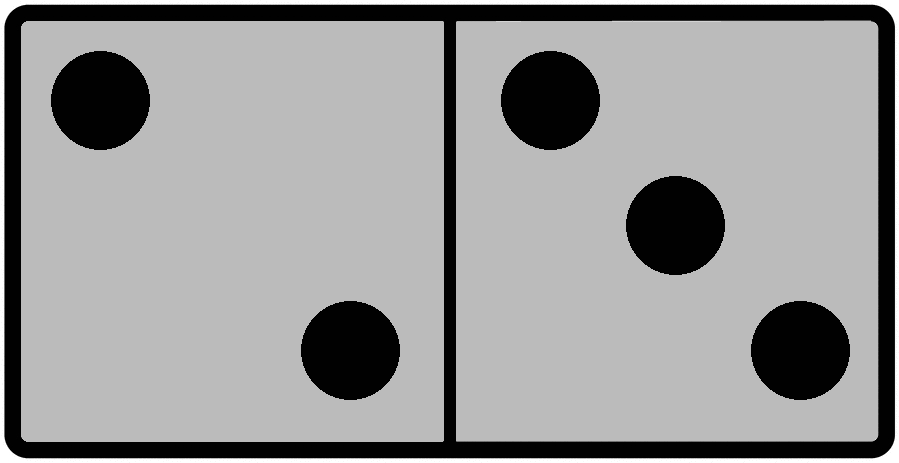
\includegraphics[width=0.3\textwidth]{gray2_3.png}
\end{center}

and your goal domino is:
\begin{center}
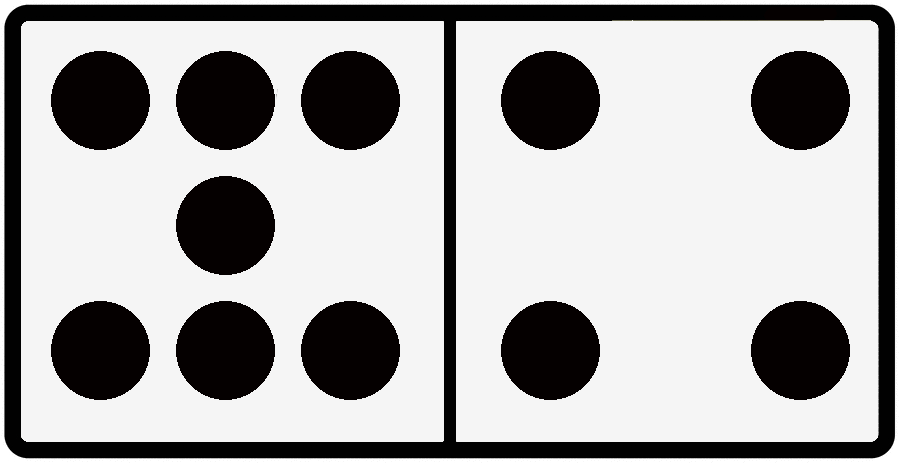
\includegraphics[width=0.3\textwidth]{white7_4.png}
\end{center}

A solution would be ``\textbf{one} and \textbf{one}.'' This means that you'll
take \textit{one} copy of the first starter domino, and \textit{one} copy of
the second, and add them together.

\begin{center}
{\LARGE Solution: \textbf{1 \& 1}}

1 \raisebox{-0.3\height}{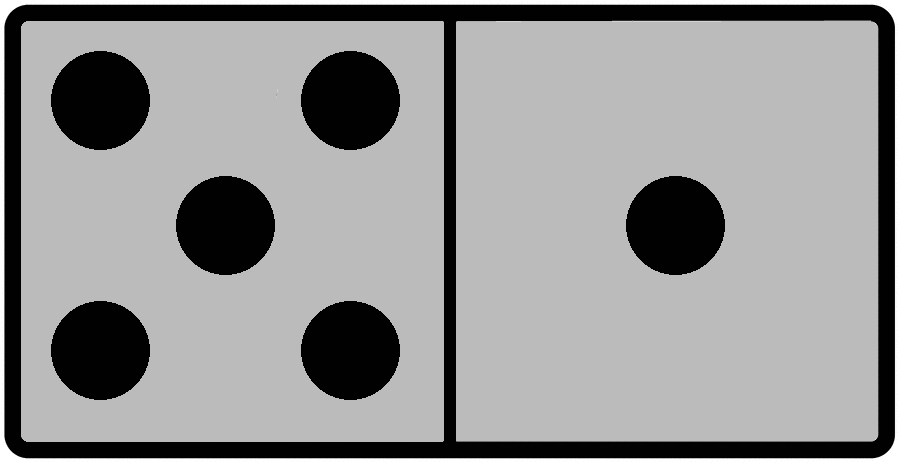
\includegraphics[width=0.1\textwidth]{gray5_1.png}} \ \& \
1 \raisebox{-0.3\height}{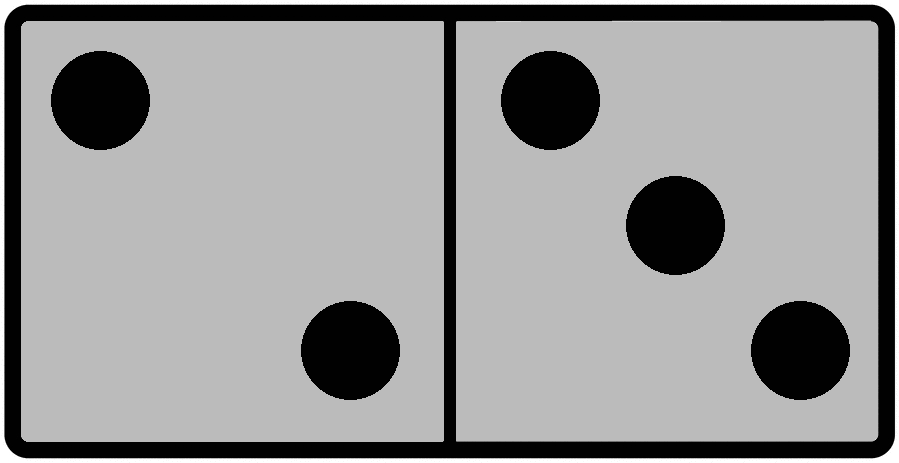
\includegraphics[width=0.1\textwidth]{gray2_3.png}} \ = \
\raisebox{-0.3\height}{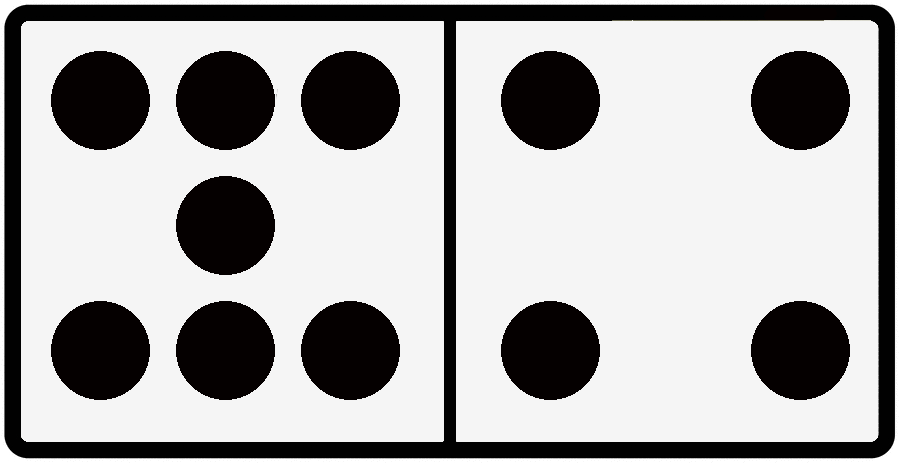
\includegraphics[width=0.1\textwidth]{white7_4.png}} \quad
\end{center}

Stare carefully at that until you master how it works; the rest of this chapter
will be a complete waste of time if this operation is not fully grasped. Adding
domino 5--1 to 2--3 means adding the left sides together, and separately adding
the right sides together, to produce a new domino 7--4 (since $5+2=7$ and
$1+3=4$).

